\section{均匀平面波对分界平面的垂直入射}
在本节,我们会讨论均匀平面波对介质间的分解平面的垂直入射,具体讨论两种情况
\begin{enumerate}
    \item 从理想介质,到理想导体的垂直入射。
    \item 从理想介质,到理想介质的垂直入射。
\end{enumerate}

\subsection{对理想导体的垂直入射}
在本小节,我们考虑如\xref{fig:对理想导体的垂直入射}所示的情形,均匀平面电磁波由理想介质入射理想导体。
\begin{Figure}[对理想导体的垂直入射]
    \includegraphics[scale=0.85]{build/Chapter06A_01.fig.pdf}
\end{Figure}
我们会问,为什么是入射理想导体?由于理想导体的电导率$\sigma=\infty$,因此事实上理想导体内不允许电场$\vb*{E}$的存在,换言之,电磁波将无法在理想导体中传播,因此,电磁波入射理想导体时,将完全被反射,而不存在透射。这样,问题分析上将简单一些,相对比较容易上手。

我们还需要指出,简单起见,假设这里的入射电磁波均为线偏振波。

\begin{BoxFormula}[对理想导体的垂直入射]
    当均匀平面电磁波垂直入射理想导体时,有
    \begin{Equation}
        E_\text{rm}=-E_\text{im}
    \end{Equation}
    其中$E_\text{im},E_\text{rm}$分别为入射电磁波和反射电磁波的振幅。

    入射电磁波的波函数为
    \begin{Equation}
        \vb*{\dot{E}}_\text{i}(z)=\vb*{e}_xE_\text{im}\e^{-\j k_1z}\qquad
        \vb*{\dot{H}}_\text{i}(z)=\vb*{e}_y\eta_1^{-1}E_\text{im}\e^{-\j k_1z}
    \end{Equation}
    反射电磁波的波函数为
    \begin{Equation}
        \vb*{\dot{E}}_\text{r}(z)=-\vb*{e}_xE_\text{im}\e^{\j k_1z}\qquad
        \vb*{\dot{H}}_\text{r}(z)=\vb*{e}_y\eta_1^{-1}E_\text{im}\e^{\j k_1z}
    \end{Equation}
\end{BoxFormula}

\begin{Proof}
    入射电磁波是向$z$轴正方向传播的均匀平面波,设为
    \begin{Equation}&[1]
        \qquad\qquad\quad
        \vb*{\dot{E}}_\text{i}(z)=\vb*{e}_xE_\text{im}\e^{-\j k_1z}\qquad
        \vb*{\dot{H}}_\text{i}(z)=+\vb*{e}_\text{z}\times\eta_1^{-1}\vb*{\dot{E}}_\text{i}(z)=\vb*{e}_y\eta_1^{-1}E_\text{im}\e^{-\j k_1z}
        \qquad\qquad\quad
    \end{Equation}
    反射电磁波是向$z$轴负方向传播的均匀平面波,设为
    \begin{Equation}&[2]
        \qquad\qquad\hspace{0.2cm}
        \vb*{\dot{E}}_\text{r}(z)=\vb*{e}_xE_\text{rm}\e^{\j k_1z}\qquad
        \vb*{\dot{H}}_\text{r}(z)=-\vb*{e}_\text{z}\times\eta_1^{-1}\vb*{\dot{E}}_\text{i}(z)=-\vb*{e}_y\eta_1^{-1}E_\text{rm}\e^{\j k_1z}
        \qquad\qquad
    \end{Equation}
    透射电磁波并不存在,因为理想导体无法传递电磁波。

    在介质1中的合成波的电场和磁场就分别为
    \begin{Gather}[6pt]
        \vb*{\dot{E}}_1(z)=\vb*{\dot{E}}_\text{i}(z)+\vb*{\dot{E}}_\text{r}(z)=\vb*{e}_x\qty(E_\text{im}\e^{-\j k_1 z}+E_\text{rm}\e^{\j k_1z})\xlabelpeq{3}\\
        \vb*{\dot{H}}_2(z)=\vb*{\dot{H}}_\text{i}(z)+\vb*{\dot{H}}_\text{r}(z)=\vb*{e}_y\eta_1^{-1}\qty(E_\text{im}\e^{-\j k_1 z}+E_\text{rm}\e^{\j k_1z})\xlabelpeq{4}
    \end{Gather}
    在介质2中,由于是理想导体,不存在电磁场(不存在透射波)
    \begin{Equation}&[5]
        \vb*{\dot{E}}_2(z)=\vb*{0}\qquad
        \vb*{\dot{H}}_2(z)=\vb*{0}
    \end{Equation}
    根据\fancyref{fml:电场强度的边界条件},电场强度的切向分量在分界面连续
    \begin{Equation}&[6]
        E_{1x}(z)=E_{2x}(z)
    \end{Equation}
    代入\xrefpeq{3}和\xrefpeq{5}得
    \begin{Equation}&[7]
        E_\text{im}+E_\text{rm}=0
    \end{Equation}
    即
    \begin{Equation}&[8]
        E_\text{rm}=-E_\text{im}
    \end{Equation}
    将\xrefpeq{8}代入\xrefpeq{2}中,即可将反射电磁波用入射电磁波的振幅$E_\text{im}$表示了。
\end{Proof}

\begin{BoxFormula}[对理想导体垂直入射时的合成波]
    当均匀平面电磁波垂直入射理想导体时,入射波和反射波的合成波为
    \begin{Equation}
        \qquad\qquad\qquad
        \vb*{\dot{E}}_1(z)=-\vb*{e}_x\j 2\vb*{E}_\text{im}\sin(k_1z)\qquad
        \vb*{\dot{H}}_1(z)=\vb*{e}_y2\eta^{-1}\vb*{E}_\text{im}\cos(k_1z)
        \qquad\qquad\qquad
    \end{Equation}
    或记作时变形式
    \begin{Gather}[6pt]
        \vb*{E}_1(z,t)=\vb*{e}_x2E_\text{im}\sin(k_1z)\sin(\omega t)\\
        \vb*{H}_1(z,t)=\vb*{e}_y2\eta_1^{-1}E_\text{im}\cos(k_1z)\cos(\omega t)
    \end{Gather}
\end{BoxFormula}

\begin{Proof}
    根据\fancyref{fml:对理想导体的垂直入射}中电场的波函数
    \begin{Equation}
        \vb*{\dot{E}}_1(z)=\vb*{\dot{E}}_\text{i}(z)+\vb*{\dot{E}}_\text{r}(z)=\vb*{e}_xE_\text{im}\qty(\e^{-\j k_1z}-\e^{\j k_1z})
    \end{Equation}
    由于$\sin\theta=(\e^{\j\theta}-\e^{-\j\theta})/2\j$
    \begin{Equation}
        \vb*{\dot{E}}_1(z)=-\vb*{e}_x2\j E_\text{im}\sin(k_1z)
    \end{Equation}
    改写为时变形式,并考虑到$-\j=\e^{-\pi/2}$和$\cos(\theta-\pi/2)=\sin(\theta)$
    \begin{Equation}
        \vb*{E}_1(z,t)=\vb*{e}_x2E_\text{im}\sin(k_1z)\sin(\omega t)
    \end{Equation}
    根据\fancyref{fml:对理想导体的垂直入射}中磁场的波函数
    \begin{Equation}
        \vb*{\dot{H}}_1(z)=\vb*{\dot{H}}_\text{i}(z)+\vb*{\dot{H}}_\text{r}(z)=\vb*{e}_y\eta^{-1}E_\text{im}\qty(\e^{-\j k_1z}+\e^{\j k_1z})
    \end{Equation}
    由于$\cos\theta=(\e^{\j\theta}+\e^{-\j\theta})/2$
    \begin{Equation}
        \vb*{\dot{H}}_1(z)=\vb*{e}_y\eta^{-1}E_\text{im}\cos(k_1z)
    \end{Equation}
    改写为时变形式
    \begin{Equation}
        \vb*{H}_1(z,t)=\vb*{e}_y2\eta_1^{-1}E_\text{im}\cos(k_1z)\cos(\omega t)
    \end{Equation}
    这就求得了入射波和反射波叠加后的合成波。
\end{Proof}

根据\xref{fml:对理想导体垂直入射时的合成波}可见,当入射波和反射波叠加后,合成波的相位仅随时间变化,空间各点相位相同(这里是$\cos(\omega t)$,与通常的$\cos(\omega t+kz)$不同),空间变化反映在振幅上。换言之,合成波在空间没有移动,只是在原来的位置以振动,故形象的称为\uwave{驻波}(Stationary Wave),与通常的\uwave{行波}(Traveling Wave)区分。驻波的振动模式如\xref{tab:驻波}所示,我们看到,在驻波中,各点的最大振幅将随空间以正弦或余弦方式分布,各点在原位随时间上下作同相位的简谐振动。

\begin{Table}[驻波]{|c|c|}
<电场驻波&磁场驻波\\>
\xcell<c>[2ex][0ex]
{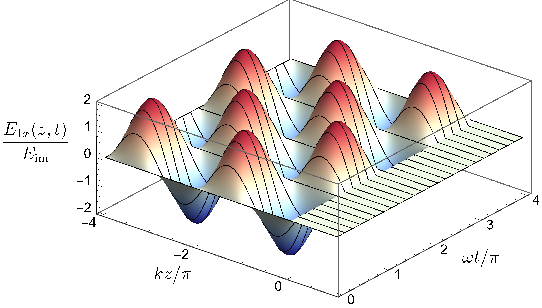
\includegraphics[width=7cm]{Mathematica/output/EReflect3D.pdf}}&
\xcell<c>[2ex][0ex]
{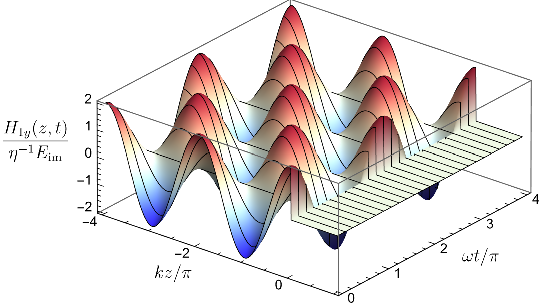
\includegraphics[width=7cm]{Mathematica/output/HReflect3D.pdf}}\\
\xcell<c>[2ex][0ex]
{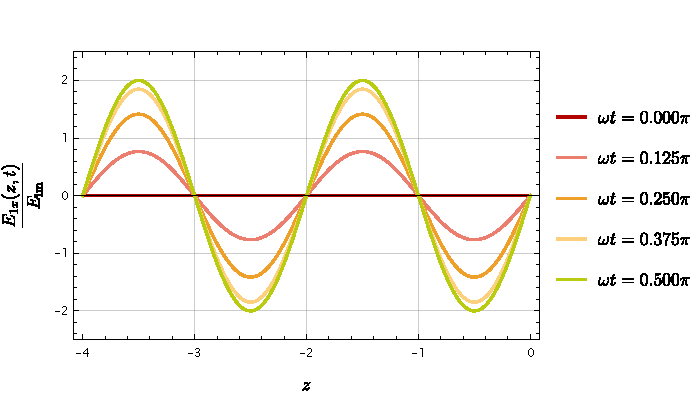
\includegraphics[width=7cm]{Mathematica/output/EReflect.pdf}}&
\xcell<c>[2ex][0ex]
{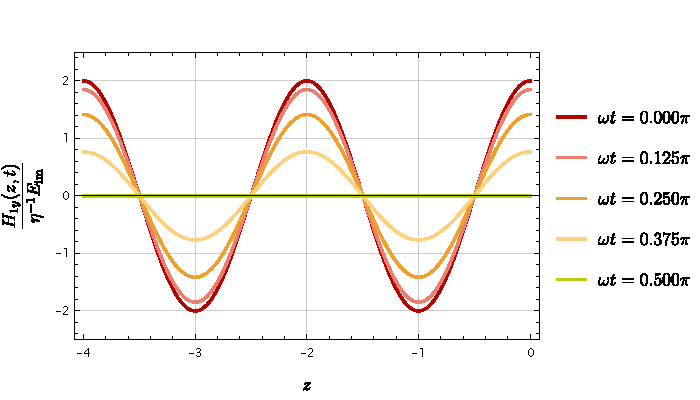
\includegraphics[width=7cm]{Mathematica/output/HReflect.pdf}}\\
\end{Table}

\begin{BoxFormula}[对理想导体垂直入射时的合成波振幅]
    当均匀平面电磁波垂直入射理想导体时,合成波的的振幅为
    \begin{Equation}
        \abs*{\vb*{\dot{E_1}}(z)}=2E_\text{im}\abs*{\sin(k_1z)}\qquad
        \abs*{\vb*{\dot{H_1}}(z)}=2\eta^{-1}E_\text{im}\abs{\cos(k_1z)}
    \end{Equation}
    当$z$为四分之一波长的偶数倍时,是合成波电场的波腹点
    \begin{Equation}
        \abs*{\vb*{\dot{E_1}}(z)}_{\max}
        =2E_\text{im}
        \qquad 
        z=-(2n)\frac{\lambda_1}{4}
    \end{Equation}
    当$z$为四分之一波长的奇数倍时,是合成波电场的波节点
    \begin{Equation}
        \abs*{\vb*{\dot{E_1}}(z)}_{\min}
        =0
        \qquad
        z=-(2n+1)\frac{\lambda_1}{4}
    \end{Equation}
\end{BoxFormula}
\begin{Proof}\nopagebreak
    根据\fancyref{fml:对理想导体垂直入射时的合成波}
    \begin{Equation}
        \vb*{\dot{E_1}}(z)=-\vb*{e}_x\j 2\vb*{E}_\text{im}\sin(k_1 z)
    \end{Equation}
    取模得
    \begin{Equation}
        |\vb*{\dot{E_1}}(z)|=2\vb*{E}_\text{im}|\sin(k_1 z)|
    \end{Equation}
    这就得到了电场的振幅,类似的也可以得到磁场的振幅。

    当$k_1z=-(2n)(\pi/2)$时,有$|\sin(k_1z)|=1$使$|\vb*{\dot{E}}_1(z)|$取最大值$2E_\text{im}$,此时
    \begin{Equation}
        z=-(2n)\frac{\pi}{2k_1}=-(2n)\frac{\lambda_1}{4}        
    \end{Equation}
    当$k_1z=-(2n+1)(\pi/2)$时,有$|\sin(k_1z)|=0$使$|\vb*{\dot{E}}_2(z)|$取最小值$0$,此时
    \begin{Equation}
        z=-(2n+1)\frac{\pi}{2k_1}=-(2n+1)\frac{\lambda_1}{4}
    \end{Equation}
    这里的关键是代入角波数$k$和波长$\lambda$间的关系$k=2\pi/\lambda$。
\end{Proof}

值得注意的是,电场的波腹点恰是磁场的波节点,电场的波节点恰是磁场的波腹点。

\begin{BoxFormula}[对理想导体垂直入射时的坡印廷矢量]
    当均匀平面电磁波垂直入射理想导体时,合成波的平均坡印廷矢量为
    \begin{Equation}
        \vb*{S}_\text{1av}=\vb*{0}
    \end{Equation}
\end{BoxFormula}

\begin{Proof}
    根据\fancyref{fml:平均坡印廷矢量}
    \begin{Equation}
        \vb*{S}_\text{1av}=\frac{1}{2}\Re\qty[\vb*{\dot{E}}_1\times\vb*{\dot{H}}_1^{*}]
    \end{Equation}
    根据\fancyref{fml:对理想导体垂直入射时的合成波}
    \begin{Equation}
        \vb*{S}_\text{1av}=\frac{1}{2}\Re\qty[-\vb*{e}_\text{z}\j 4\eta^{-1}E_\text{im}^2\sin(k_1z)\cos(k_1z)]
    \end{Equation}
    注意到这里只存在虚部,因此
    \begin{Equation}*
        \vb*{S}_\text{1av}=\vb*{0}\qedhere
    \end{Equation}
\end{Proof}
\fancyref{fml:对理想导体垂直入射时的坡印廷矢量}表明
\begin{itemize}
    \item 驻波不发生电磁能量的传输。
    \item 驻波仅在两个波节间进行电场能量和磁场能量的交换。
\end{itemize}

是否在空间上传播电磁能量,是区分该电磁波是行波还是驻波的一个重要特征。

\subsection{对理想介质的垂直入射}
在本小节,我们考虑如\xref{fig:对理想介质的垂直入射}所示的情形,均匀平面电磁波由理想介质入射理想介质。
\begin{Figure}[对理想介质的垂直入射]
    \includegraphics[scale=0.85]{build/Chapter06A_02.fig.pdf}
\end{Figure}
这时,入射后会同时产生反射波和透射波,情况会变复杂些。

\begin{BoxFormula}[对理想介质的垂直入射]*
    当均匀平面电磁波垂直入射理想介质时,有
    \begin{Equation}
        E_\text{rm}=RE_\text{im}\qquad
        E_\text{tm}=TE_\text{tm}
    \end{Equation}
    其中$E_\text{im},E_\text{rm},E_\text{tm}$分别为入射、反射、折射电磁波的振幅。

    系数$R$称为\uwave{反射系数}(Reflection Coefficient),满足
    \begin{Equation}
        R=\frac{E_\text{rm}}{E_\text{im}}=\frac{\eta_2-\eta_1}{\eta_2+\eta_1}
    \end{Equation}
    系数$T$称为\uwave{透射系数}(Transmission Coefficient),满足
    \begin{Equation}
        T=\frac{E_\text{tm}}{E_\text{im}}=1+R=\frac{2\eta_2}{\eta_2+\eta_1}
    \end{Equation}
    入射电磁波的波函数为
    \begin{Equation}
        \vb*{\dot{E}}_\text{i}(z)=\vb*{e}_xE_\text{im}\e^{-\j k_1z}\qquad
        \vb*{\dot{H}}_\text{i}(z)=\vb*{e}_y\eta_1^{-1}E_\text{im}\e^{-\j k_1z}
    \end{Equation}
    反射电磁波的波函数为
    \begin{Equation}
        \vb*{\dot{E}}_\text{t}(z)=\vb*{e}_xRE_\text{im}\e^{\j k_1z}\qquad
        \vb*{\dot{H}}_\text{t}(z)=-\vb*{e}_y\eta_1^{-1}RE_\text{im}\e^{\j k_1z}
    \end{Equation}
    透射电磁波的波函数为
    \begin{Equation}
        \vb*{\dot{E}}_\text{t}(z)=\vb*{e}_xTE_\text{im}\e^{-\j k_2z}\qquad
        \vb*{\dot{H}}_\text{t}(z)=\vb*{e}_y\eta_1^{-1}TE_\text{im}\e^{-\j k_2z}
    \end{Equation}
\end{BoxFormula}

\begin{Proof}
    入射电磁波是在介质1中,向$z$轴正方向传播的均匀平面波,设为
    \begin{Equation}&[1]
        \qquad\qquad\quad
        \vb*{\dot{E}}_\text{i}(z)=\vb*{e}_xE_\text{im}\e^{-\j k_1z}\qquad
        \vb*{\dot{H}}_\text{i}(z)=+\vb*{e}_\text{z}\times\eta_1^{-1}\vb*{\dot{E}}_\text{i}(z)=\vb*{e}_y\eta_1^{-1}E_\text{im}\e^{-\j k_1z}
        \qquad\qquad\quad
    \end{Equation}
    反射电磁波是在介质1中,向$z$轴负方向传播的均匀平面波,设为
    \begin{Equation}&[2]
        \qquad\qquad\hspace{0.2cm}
        \vb*{\dot{E}}_\text{r}(z)=\vb*{e}_xE_\text{rm}\e^{\j k_1z}\qquad
        \vb*{\dot{H}}_\text{r}(z)=-\vb*{e}_\text{z}\times\eta_1^{-1}\vb*{\dot{E}}_\text{i}(z)=-\vb*{e}_y\eta_1^{-1}E_\text{rm}\e^{\j k_1z}
        \qquad\qquad
    \end{Equation}
    透射电磁波是在介质2中,向$z$轴正方向传播的均匀平面波,设为
    \begin{Equation}&[3]
        \qquad\qquad\quad
        \vb*{\dot{E}}_\text{t}(z)=\vb*{e}_xE_\text{tm}\e^{-\j k_2z}\qquad
        \vb*{\dot{H}}_\text{t}(z)=+\vb*{e}_\text{z}\times\eta_1^{-1}\vb*{\dot{E}}_\text{i}(z)=\vb*{e}_y\eta_1^{-1}E_\text{tm}\e^{-\j k_2z}
        \qquad\qquad\quad
    \end{Equation}
    介质1中的电磁波是入射和反射的叠加
    \begin{Gather}[6pt]
        \vb*{\dot{E}}_1(z)=\vb*{\dot{E}}_\text{i}(z)+\vb*{\dot{E}}_\text{r}(z)=\vb*{e}_x\qty(E_\text{im}\e^{-\j k_1 z}+E_\text{rm}\e^{\j k_1z})\xlabelpeq{4}\\
        \vb*{\dot{H}}_1(z)=\vb*{\dot{H}}_\text{i}(z)+\vb*{\dot{H}}_\text{r}(z)=\vb*{e}_y\eta_1^{-1}\qty(E_\text{im}\e^{-\j k_1 z}+E_\text{rm}\e^{\j k_1z})\xlabelpeq{5}
    \end{Gather}
    介质2中的电磁波仅包含透射部分
    \begin{Gather}[6pt]
        \vb*{\dot{E}}_2(z)=\vb*{\dot{E}}_\text{t}(z)=\vb*{e}_xE_\text{tm}\e^{-\j k_2z}\xlabelpeq{6}\\
        \vb*{\dot{H}}_2(z)=\vb*{\dot{H}}_\text{t}(z)=\vb*{e}_y\eta_1^{-1}E_\text{tm}\e^{-\j k_2z}\xlabelpeq{7}
    \end{Gather}
    根据\fancyref{fml:电场强度的边界条件},电场强度的切向分量在分界面连续
    \begin{Equation}&[8]
        E_{1x}(z)=E_{2x}(z)
    \end{Equation}
    根据\fancyref{fml:磁场强度的边界条件},磁场强度的法向分量在分界面连续
    \begin{Equation}&[9]
        H_{1y}(z)=H_{2y}(z)
    \end{Equation}
    即得
    \begin{Equation}&[10]
        E_\text{im}+E_\text{rm}=E_\text{tm}\qquad
        E_\text{im}\eta_1^{-1}-
        E_\text{rm}\eta_1^{-1}=
        E_\text{tm}\eta_2^{-1}
    \end{Equation}
    将右式两端同乘$\eta_1\eta_2$
    \begin{Equation}&[11]
        E_\text{im}+E_\text{rm}=E_\text{tm}\qquad
        E_\text{im}\eta_2-
        E_\text{rm}\eta_2=
        E_\text{tm}\eta_1
    \end{Equation}
    \subparagraph{求出$E_\textnormal{rm}$与$E_\textnormal{im}$的关系}将\xrefpeq{11}的左式代入右式,以$E_\text{tm}=E_\text{rm}+E_\text{im}$作代换
    \begin{Equation}&[12]
        E_\text{im}\eta_2-E_\text{rm}\eta_2=(E_\text{im}+E_\text{rm})\eta_1
    \end{Equation}
    整理得
    \begin{Equation}&[13]
        E_\text{im}(\eta_2-\eta_1)=E_\text{rm}(\eta_2+\eta_1)
    \end{Equation}
    即
    \begin{Equation}&[14]
        E_\text{rm}=\frac{\eta_2-\eta_1}{\eta_2+\eta_1}E_\text{im}
    \end{Equation}
    \subparagraph{求出$E_\textnormal{tm}$和$E_\textnormal{im}$的关系} 将\xrefpeq{11}的左式代入右式,将$E_\text{rm}=E_\text{tm}-E_\text{im}$代换掉
    \begin{Equation}&[13]
        E_\text{im}\eta_2-(E_\text{tm}-E_\text{im})\eta_2=E_\text{tm}\eta_1
    \end{Equation}
    整理得
    \begin{Equation}
        E_\text{im}2\eta_2=E_\text{tm}(\eta_2+\eta_1)
    \end{Equation}
    即
    \begin{Equation}
        E_\text{tm}=\frac{2\eta_2}{\eta_2+\eta_1}E_\text{im}
    \end{Equation}
    将反射振幅$E_\text{rm}$和透射振幅$E_\text{tm}$与入射振幅$E_\text{im}$的比,记作反射系数$R$和透射系数$T$
    \begin{Equation}
        R=\frac{E_\text{rm}}{E_\text{im}}=\frac{\eta_2-\eta_1}{\eta_2+\eta_1}\qquad
        T=\frac{E_\text{tm}}{E_\text{im}}=\frac{2\eta_2}{\eta_2+\eta_1}
    \end{Equation}
    而很显然的
    \begin{Equation}
        R+1=\frac{\eta_2-\eta_2}{\eta_2+\eta_1}+1=\frac{2\eta_2}{\eta_2+\eta_1}=T
    \end{Equation}
    这就得到了反射系数和透射系数的表达式了。
\end{Proof}
反射系数$R=(\eta_2-\eta_1)/(\eta_2+\eta_1)$的取值范围是$R\in [-1,1]$
\begin{itemize}
    \item 当$\eta_1<\eta_2$时(波疏至波密),反射系数$R>0$,反射波与入射波相位相同。
    \item 当$\eta_1>\eta_2$时(波密至波疏),反射系数$R<0$,反射波与入射波相位相反。
\end{itemize}
透射系数$T=(\eta_2-\eta_1)/(\eta_2+\eta_1)$的取值范围是$T\in [0,2]$
\begin{itemize}
    \item 当$\eta_1<\eta_2$时(波疏至波密),透射系数$T>1$,透射波与入射波同相位,振幅更强。
    \item 当$\eta_1>\eta_2$时(波密至波疏),透射系数$T<1$,透射波与入射波同相位,振幅更弱。
\end{itemize}
所谓相位相反,就是指相位发生了$\pi$的跃变,而相位$\pi$对应半波长,因此这种现象被形象的称为\uwave{半波损失}(Half Wave Loss)。由以上讨论,我们可以看出,半波损失只会在波密至波疏的反射波中出现,透射波无论介质波阻抗关系如何,总是与入射波同相位,不发生半波损失。

\begin{BoxFormula}[对理想介质垂直入射的合成波]
    当均匀平面电磁波垂直入射理想介质时,入射波和反射波的合成波为
    \begin{Gather}[6pt]
        \vb*{\dot{E}}_1(z)=\vb*{e}_xE_\text{im}\qty[(1-R)\e^{-\j k_1z}+2R\cos(k_1z)]\\
        \vb*{\dot{H}}_1(z)=\vb*{e}_y\eta_1^{-1}E_\text{im}\qty[(1-R)\e^{-\j k_1z}-\j 2R\cos(k_1z)]
    \end{Gather}
\end{BoxFormula}

\begin{Proof}
    根据\fancyref{fml:对理想介质垂直入射的合成波}中电场的波函数
    \begin{Equation}
        \vb*{\dot{E}}_1(z)=
        \vb*{\dot{E}}_\text{i}(z)+
        \vb*{\dot{E}}_\text{r}(z)=
        \vb*{e}_xE_\text{im}\qty(\e^{-\j k_1z}+R\e^{\j k_1z})
    \end{Equation}
    做一些整理
    \begin{Equation}
        \vb*{\dot{E}}_1(z)=
        \vb*{e}_xE_\text{im}
        \qty[(1-R)\e^{-\j k_1z}+R(\e^{-\j k_1z}+\e^{\j k_1z})]
    \end{Equation}
    应用$\cos\theta=(\e^{\j\theta}+\e^{-\j\theta})/2$
    \begin{Equation}
        \vb*{\dot{E}}_1(z)=
        \vb*{e}_xE_\text{im}
        \qty[(1-R)\e^{-\j k_1z}+2R\cos(k_1z)]
    \end{Equation}
    根据\fancyref{fml:对理想介质垂直入射的合成波}中磁场的波函数
    \begin{Equation}
        \vb*{\dot{H}}_1(z)=
        \vb*{\dot{H}}_\text{i}(z)+
        \vb*{\dot{H}}_\text{r}(z)=
        \vb*{e}_y\eta^{-1}E_\text{im}\qty(\e^{-\j k_1z}-R\e^{\j k_1z})
    \end{Equation}
    做一些整理
    \begin{Equation}
        \vb*{\dot{H}}_1(z)=
        \vb*{e}_y\eta^{-1}E_\text{im}
        \qty[(1-R)\e^{-\j k_1z}+R(\e^{-\j k_1z}-\e^{\j k_1z})]
    \end{Equation}
    应用$\sin\theta=(\e^{\j\theta}-\e^{-\j\theta})/2\j$
    \begin{Equation}
        \vb*{\dot{H}}_1(z)=
        \vb*{e}_y\eta^{-1}E_\text{im}
        \qty[(1-R)\e^{-\j k_1z}-\j 2R\sin(k_1z)]
    \end{Equation}
    这就得到了$\vb*{\dot{E}}_1(z)$和$\vb*{\dot{H}}_1(z)$的表达式。
\end{Proof}

根据\fancyref{fml:对理想介质垂直入射的合成波},当垂直入射理想介质时,入射波和反射波的合成波电场中包含两部分,第一部分是振幅为$(1-R)E_\text{im}$沿$+z$方向的行波,第二部分是振幅为$2RE_\text{im}$的驻波,我们将这种,既有行波成分又有驻波成分的波,称为\uwave{行驻波}。

\begin{BoxFormula}[对理想介质垂直入射的合成波的振幅]
    当均匀平面电磁波垂直入射理想介质时,合成波的振幅为
    \begin{Equation}
        \abs*{\vb*{\dot{E}}_1(z)}=E_\text{im}\sqrt{1+R^2+2R\cos(2k_1z)}
    \end{Equation}
    最大值为
    \begin{Equation}
        \qquad
        |\vb*{\dot{E}}_1(z)|=E_\text{im}(1+|R|)\qquad z=-(2n)\frac{\lambda_1}{4}, (R>0)\qquad z=-(2n+1)\frac{\lambda_1}{4}, (R<0)
        \qquad
    \end{Equation}
    最小值为
    \begin{Equation}
        \qquad
        |\vb*{\dot{E}}_1(z)|=E_\text{im}(1-|R|)\qquad z=-(2n+1)\frac{\lambda_1}{4}, (R>0)\qquad z=-(2n)\frac{\lambda_1}{4}, (R<0)
        \qquad
    \end{Equation}
\end{BoxFormula}


\begin{Proof}
    根据\fancyref{fml:对理想介质垂直入射的合成波}
    \begin{Equation}&[1]
        |\vb*{\dot{E}}_1(z)|=E_\text{im}\abs{(1-R)\e^{-\j k_1z}+2R\cos(k_1 z)\vphantom{A^2}}
    \end{Equation}
    这里求模的关键技巧是将$\e^{-\j k_1z}$展开为三角函数
    \begin{Equation}&[2]
        \qquad\qquad
        |\vb*{\dot{E}}_1(z)|=E_\text{im}\abs{(1-R)\cos(k_1z)+\j(1-R)\sin(k_1z)+2R\cos(k_1z)\vphantom{A^2}}
        \qquad\qquad
    \end{Equation}
    整理得到
    \begin{Equation}&[3]
        |\vb*{\dot{E}}_1(z)|=E_\text{im}\abs{(1+R)\cos(k_1z)+\j(1-R)\sin(k_1z)\vphantom{A^2}}
    \end{Equation}
    这样就化为了实部加虚部的形式
    \begin{Equation}&[4]
        |\vb*{\dot{E}}_1(z)|=\sqrt{(1+R)^2\cos^2(k_1z)+(1-R)^2\sin^2(k_1 z)}
    \end{Equation}
    很明显
    \begin{Equation}&[5]
        |\vb*{\dot{E}}_1(z)|=\sqrt{1+R^2+2R\qty[\cos^2(k_1z)-\sin^2(k_1z)]}
    \end{Equation}
    运用$\cos^2\theta-\sin^2\theta=\cos(2\theta)$
    \begin{Equation}
        |\vb*{\dot{E}}_1(z)|=\sqrt{1+R^2+2R\cos(2k_1z)}
    \end{Equation}
    这里关于最大值和最小值的讨论与之前相似的,不再赘述。
\end{Proof}
在工程上,常用驻波系数或驻波比$S$来描述合成波的特性,它的定义是
\begin{BoxDefinition}[驻波比]
    \uwave{驻波比}(Standing Wave Ratio)定义为合成波电场的最大值与最小值的比
    \begin{Equation}
        S=\frac{\abs*{\vb*{\dot{E}}_1}_{\max}}{\abs*{\vb*{\dot{E}}_1}_{\min}}
    \end{Equation}
\end{BoxDefinition}

\begin{BoxFormula}[对理想介质垂直入射的合成波的驻波比]
    当均匀平面电磁波垂直入射理想介质时,合成波的驻波比为
    \begin{Equation}
        S=\frac{1+|R|}{1-|R|}
    \end{Equation}
    亦可以反过来表示
    \begin{Equation}
        |R|=\frac{S-1}{S+1}
    \end{Equation}
\end{BoxFormula}

\begin{Proof}
    根据\fancyref{def:驻波比}和\fancyref{fml:对理想介质垂直入射的合成波的振幅}
    \begin{Equation}
        S=\frac{E_\text{im}(1+|R|)}{E_\text{im}(1-|R|)}=\frac{1+|R|}{1-|R|}
    \end{Equation}
    两边同乘$1-|R|$
    \begin{Equation}
        S-S|R|=1+|R|
    \end{Equation}
    整理得
    \begin{Equation}
        |R|(1+S)=(1-S)
    \end{Equation}
    即
    \begin{Equation}*
        |R|=\frac{1-S}{1+S}\qedhere
    \end{Equation}
\end{Proof}

\begin{BoxFormula}[对理想介质垂直入射的坡印廷矢量]
    当均匀平面电磁波垂直入射理想介质时,关于平均坡印廷矢量

    介质1中的平均坡印廷矢量为
    \begin{Equation}
        S_\text{1av}=\vb*{e}_z\frac{E_\text{im}^2}{2\eta_1}(1-R^2)
    \end{Equation}
    介质2中的平均坡印廷矢量为
    \begin{Equation}
        S_\text{2av}=\vb*{e}_z\frac{E_\text{im}^2}{2\eta_2}T^2
    \end{Equation}
    并且
    \begin{Equation}
        S_\text{1av}=S_\text{2av}
    \end{Equation}
\end{BoxFormula}

\begin{Proof}
    证明从略。
\end{Proof}